\documentclass[10pt, a4paper]{article}

\usepackage[a4paper, top=0.5cm, bottom=0.5cm, left=0.5cm, right=0.5cm, landscape]{geometry}
\usepackage{mathtools}
\usepackage{amsfonts}
\usepackage{multicol}
\usepackage{setspace}
\usepackage{graphicx}



\author{Zach}
\date{3 November 2020}
\setstretch{1.25}

\begin{document}
	\scriptsize %tiny
	\setlength\parindent{0pt}
	\setlength{\columnseprule}{0.1pt}
	
	\begin{center}
		{\large CS2040S CheatSheet}\\
		by Zachary Chua
	\end{center}
	
	\begin{multicols*}{3}
		
		{\normalsize\textbf{Searching and Sorting}}\\
		\textbf{Binary Search} \\
		Can be used for any monotonic function, not necessarily just for searching for number in array\\
		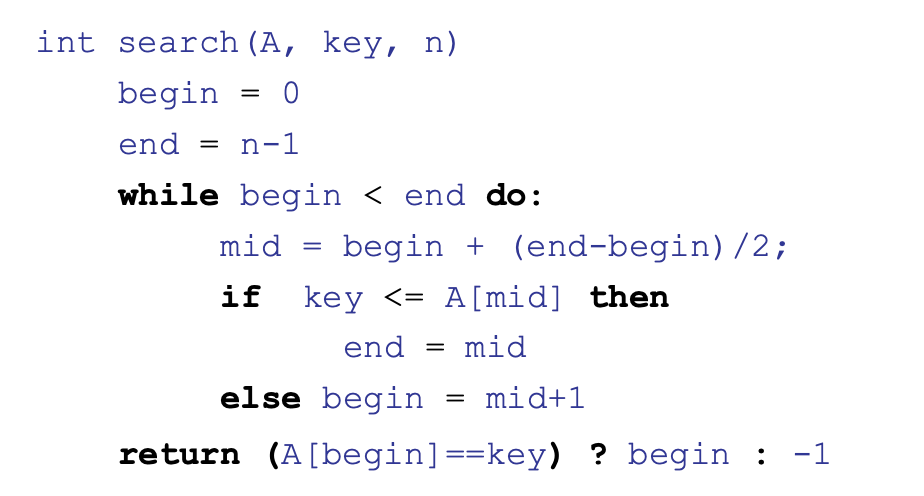
\includegraphics[scale = .3]{./assets/BinSearch.png}\\
		\textbf{Peak Finding}\\
		For finding local peak - Binary Search + recurse on larger side\\ 
		\textbf{Sorts}\\
		- BubbleSort: $\Omega(n)$ already sorted, $O(n^2)$, stable\\
		- SelectionSort: $\Omega(n^2)$, $O(n^2)$, not stable\\
		- InsertionSort: $\Omega(n)$ already sorted, $O(n^2)$ reverse order, stable\\
		- MergeSort: $O(nlogn)$, $T(n) = 2T(\frac{n}{2} + O(n)$, stable if merge step is stable.\\
		\textbf{QuickSort}\\
		Deterministic: $O(n^2)$ for worst case (sorted), $O(nlogn)$ best case.\\
		Random: $O(nlogn)$ for worst and best case.\\
		Paranoid random: Expected 2 tries.\\
		Can make stable with extra $O(n)$ space.\\
		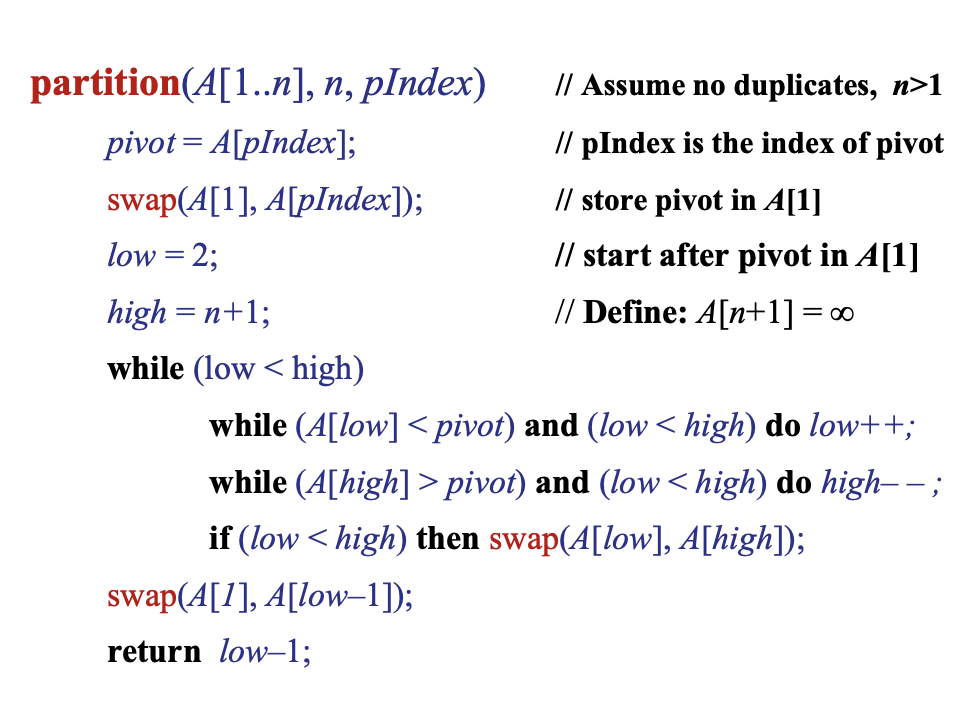
\includegraphics[scale = .27]{./assets/Partition}\\
		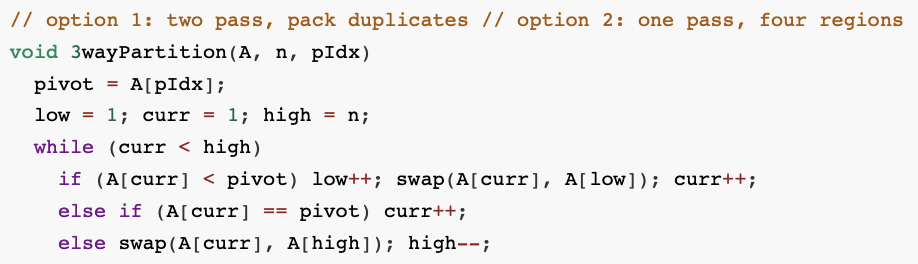
\includegraphics[scale=.4]{./assets/Partition3}\\
		\textbf{QuickSelect}\\
		Select the kth element, runtime = $O(n)$\\
		1. Partition then recurse into the correct side.\\
		2. When recursing into right half need to take note of index, $(k - i)$ where i is the index of the partition.\\ 
	
		{\normalsize\textbf{Trees}}\\
		\textbf{Tree Operations}\\
		- insert: $O(h)$, only insert at leaves\\
		- delete: $O(h)$, no child just delete, 1 child join parent and child, 2 children swap with successor and delete\\
		- successor (predecessor): $O(h)$, minimal element on right subtree or walk up tree until it is a left child. \\
		\textbf{AVL trees}\\
		Augmentation: store $v.height = max(v.left.height, v.right.height) + 1$\\
		Balance Condition: $|v.left.height - v.right.height| \leq 1$\\
		Balanced tree with n nodes has
		$h < 2logn$\\ and any balanced tree with height h has $ n > 2^{\frac{h}{2}}$\\
		\textbf{Rotation}\\
		1. Left heavy\\
		1.1 Balanced or Left-heavy: right-otation\\
		1.2 Right-heavy: Left-rotate left child then right-rotation\\
		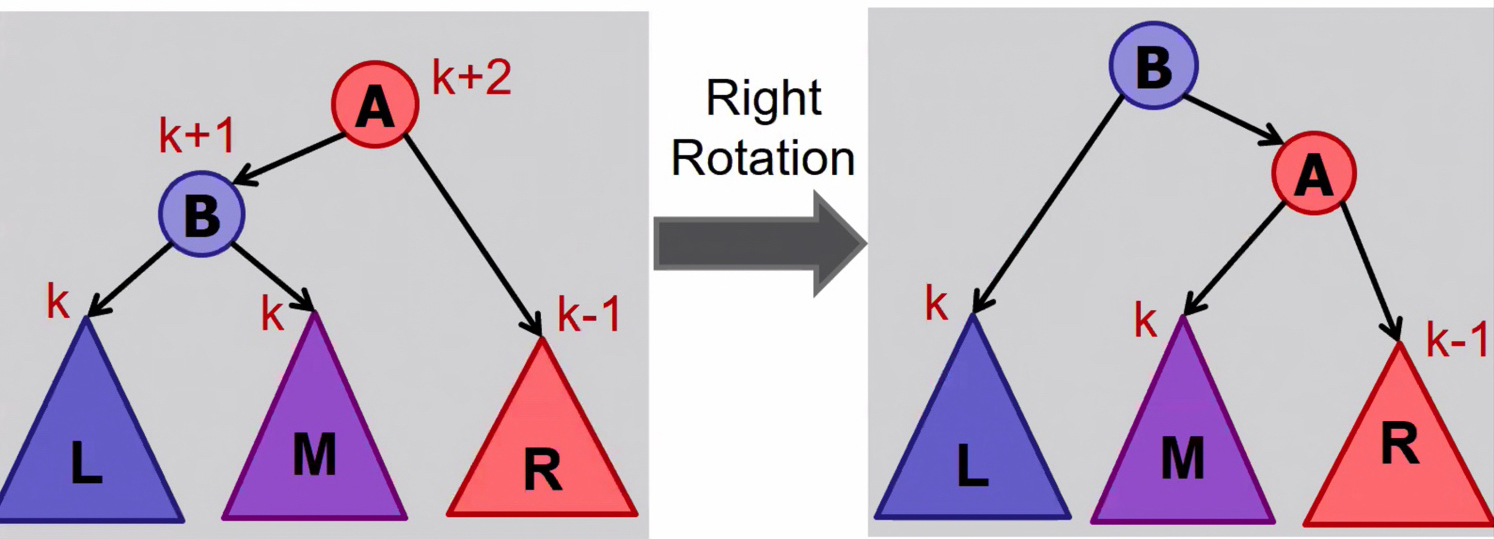
\includegraphics[scale=.07]{./assets/Rotation}\\
		Insertions: $\leq$ 2 rotations, Deletions: $O(logn)$ rotations(walk up to root)\\
		\textbf{Trie} - Search: $O(L)$ Insert: $O(L + Overhead)$\\
		Useful for prefix, longest prefix, wildcard queries\\
		\textbf{Augmented Tree}\\
		Order Statistics Tree - weights $v.weight = v.left.weight + v.right.weight + 1$ and parent pointers\\
		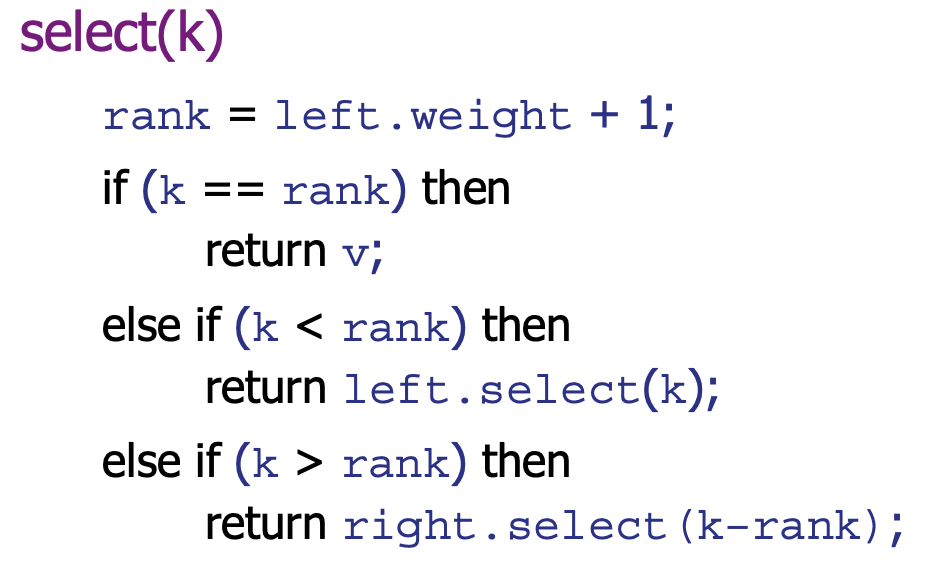
\includegraphics[scale=0.25]{./assets/Select} 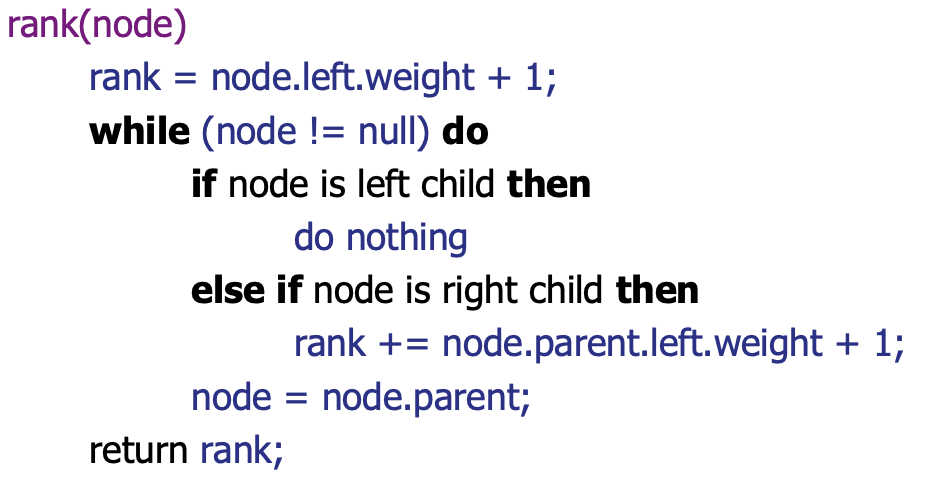
\includegraphics[scale=.3]{./assets/rank}\\
		Interval Tree - Keyed by left edge, hold max endpoint in subtree in node\\
		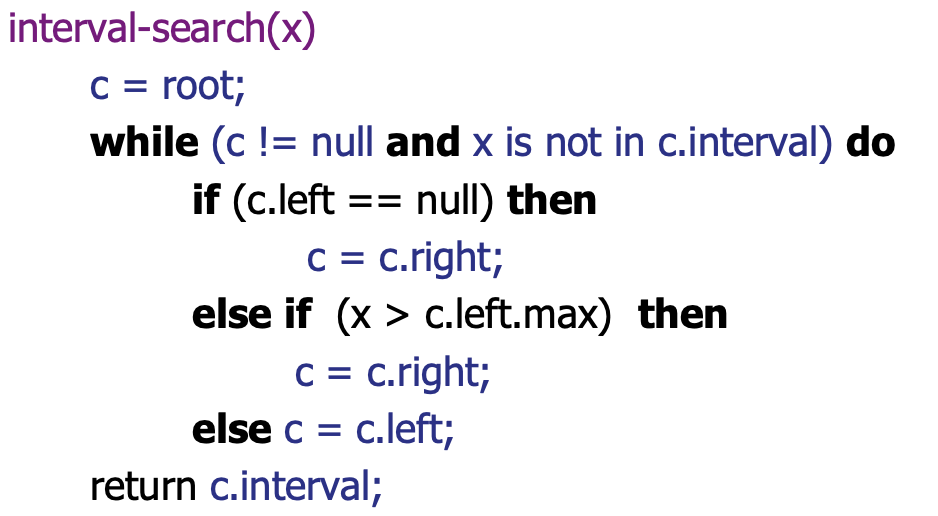
\includegraphics[scale=.25]{./assets/Interval}\\
		Orthogonal Range Finding - nodes are max value in left subtree, values are stored at leaves $O(k + logn)$, where $k$ is the number of points found.\\
		- Find split node, LeftTraversal on node.left, RightTraversal on node.right\\
		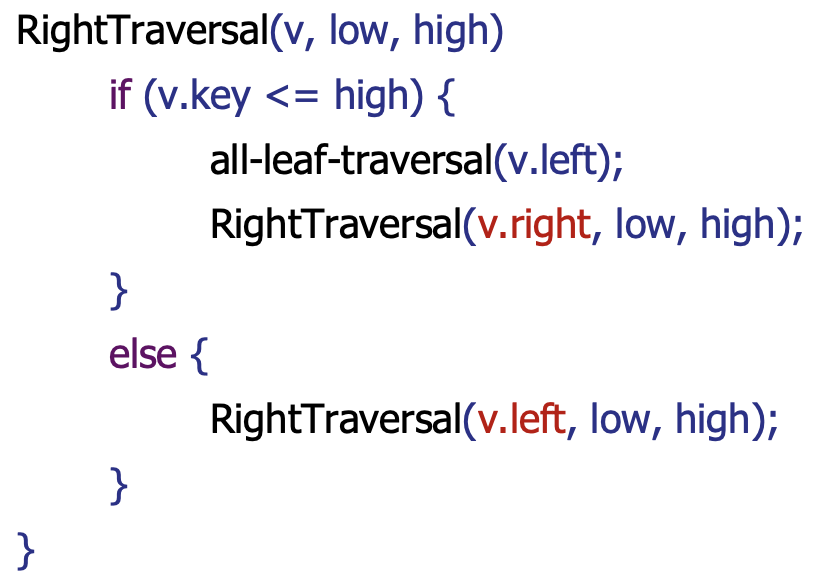
\includegraphics[scale=.25]{./assets/RightTraversal} 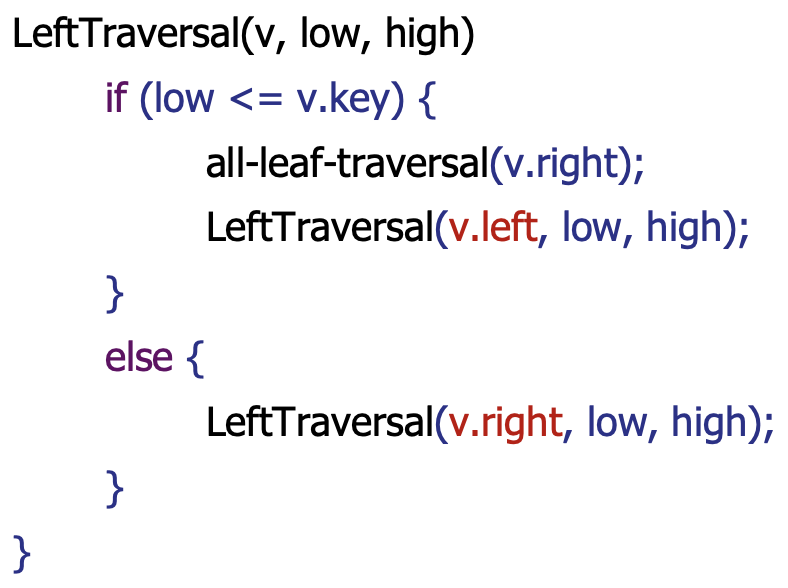
\includegraphics[scale=.25]{./assets/LeftTraversal}\\
		\textbf{$(a, b)$ trees} - B-trees are (B, 2B) trees.\\
		1. Root $[2, b]$ children, $[1, b-1]$ keys; Internal $[a, b]$ children, $[a - 1, b - 1]$ keys; Leaf 0 children, $[a - 1, b - 1]$ keys\\ 
		2. Non-leaf node must have one more child than number of keys (ensures all ranges covered by children)\\
		3. All leaf nodes must be at same depth\\
		Proactive Split - when node's keylist size = b - 1, push median key up (before parent key) and split keylist. Left keylist becomes median node's child, median node's child becomes left keylist rightmost child.\\
		Proactive Merge / Share - when node's keylist $= a - 1$, delete parent key and put between two neighbour keylists, delete the resulting empty keylist (from merging one into other). If keylist is now $>= b - 1$, split (Share).\\
	
		{\normalsize\textbf{Hashing}}\\
		Implement symbol table - key, value pairs without ordering.\\
		Search and Insert - $O(1)$\\
		\textbf{Collision resolution}\\
		Collision if $h(k_1) = h(k_2), k_1 \neq k_2$\\ 
		\textbf{Chaining} - bucket contains list, add to list if collide\\
		Insertion: $O(1 + cost(h))$, insert at front of LL\\
		Search: $O(n + cost(h))$\\
		Assuming SUHA (every key has equal chance of hashing to any bucket), \\
		Expected Search = $1 + \frac{n}{m}$ (expected no. of items per bucket), 1 for hashing and accessing hashtable.\\
		\textbf{Open Addressing} - finding another bucket\\
		For an item k, in a hashtable with m elements, on the nth try,\\
		- Linear probing: $h(k, n) = h(k) + n \mod m$\\
		- Double Hashing: $h(k, n) = h(k) + n*g(k) \mod m$, if g(k) is coprime to m, then $h(k, n)$ will hit all buckets\\ 
		Good Hash Function:\\ 
		- enumerate all possible buckets (permutation of buckets)\\
		- UHA: every key is equally likely to be mapped to every permutation, indep of other keys (NOT linear probing)\\
		Operations' cost: $\leq \frac{1}{1 - \alpha}$, assuming UHA.\\
		\textbf{Table Resizing}\\
		Increasing Table Size:\\
		1. Increment by 1: Each insert is $O(n + 1)$, overall cost of inserting n items: $O(n^2)$.\\
		2. Double Table Size: Each time resize $(O(n))$, would have inserted $O(n)$ items, amortized cost of n inserts: $O(n)$.\\
		3. Square Table Size: resizing becomes $O(n^2)$, avg cost of insert $O(n)$, inefficient space usage.\\
		Decreasing Table Size:\\
		1. Halve, $n < m/2$: Consecutive insert, delete on table size n, with n items $\rightarrow$ each operation $O(n)$\\
		2. Halve, $n < m/4$: $O(n)$ operations between resizes, Amortized cost $O(1)$\\
		Amortized Cost - Operation has amortized cost $T(n)$ if for every integer $k$, the cost of $k$ operations is $\leq kT(n)$.\\
		\textbf{Sets - FHT, Bloom Filters} - Space and Speed critical\\
		FingerprintHash Table - Only stores $0 / 1$ in HT instead of keys (save space)\\
		Collision (Insertion)- just leave table entry as 1\\
		Look up - might false positive; 2 items hash to same bucket, 1 in table, 1 not, both reflect present as bucket == 1\\
		Bloom Filter - $> 1$ hash functions, need more space: $k$ functions, $k * n$ bits.\\
		Requires all $k$ buckets = 1 for item present, reduces collisions and false +ve\\
		
		{\normalsize\textbf{Graphs}}\\
		Adjacency List (store outgoing edges in directed graphs) - sparse graph less space, fast find any nbr/ enum all nbr\\
		Adjacency Matrix - fast query if two nodes are connected\\
		\textbf{Searching Graph} - DFS, BFS explores all nodes, edges but not all paths.\\
		BFS - $O(V + E)$, can be used for unweighted, graphs w same weight, trees\\
		Returns shortest path graph from source to all nodes.\\
		%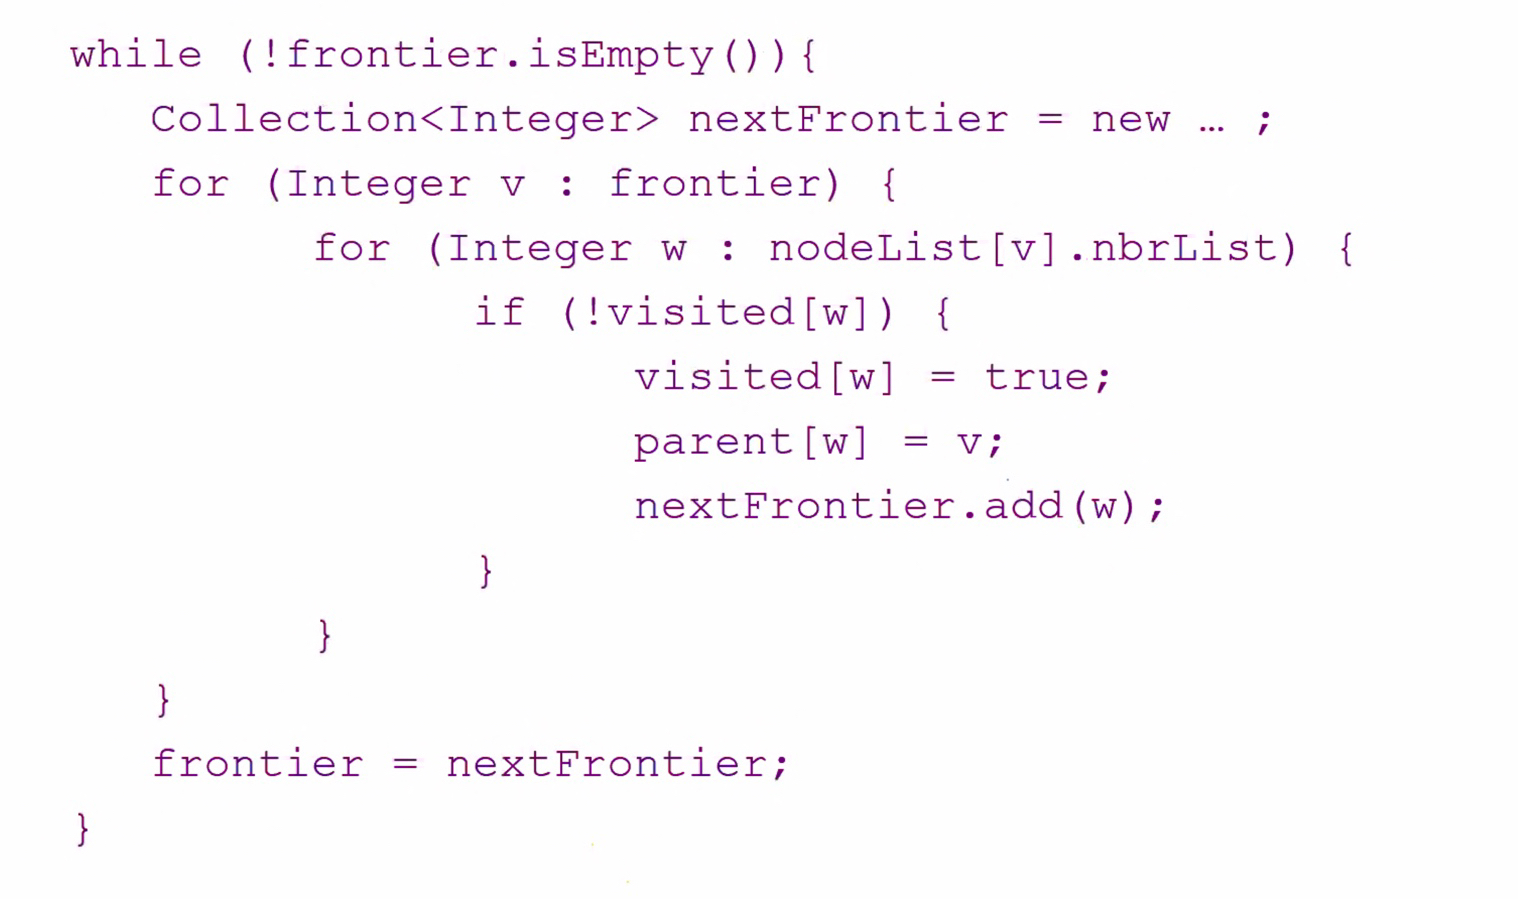
\includegraphics[scale=.12]{BFS2}\\
		DFS - $O(V + E)$, can be used for unweighted, graphs w same weight, trees\\
		%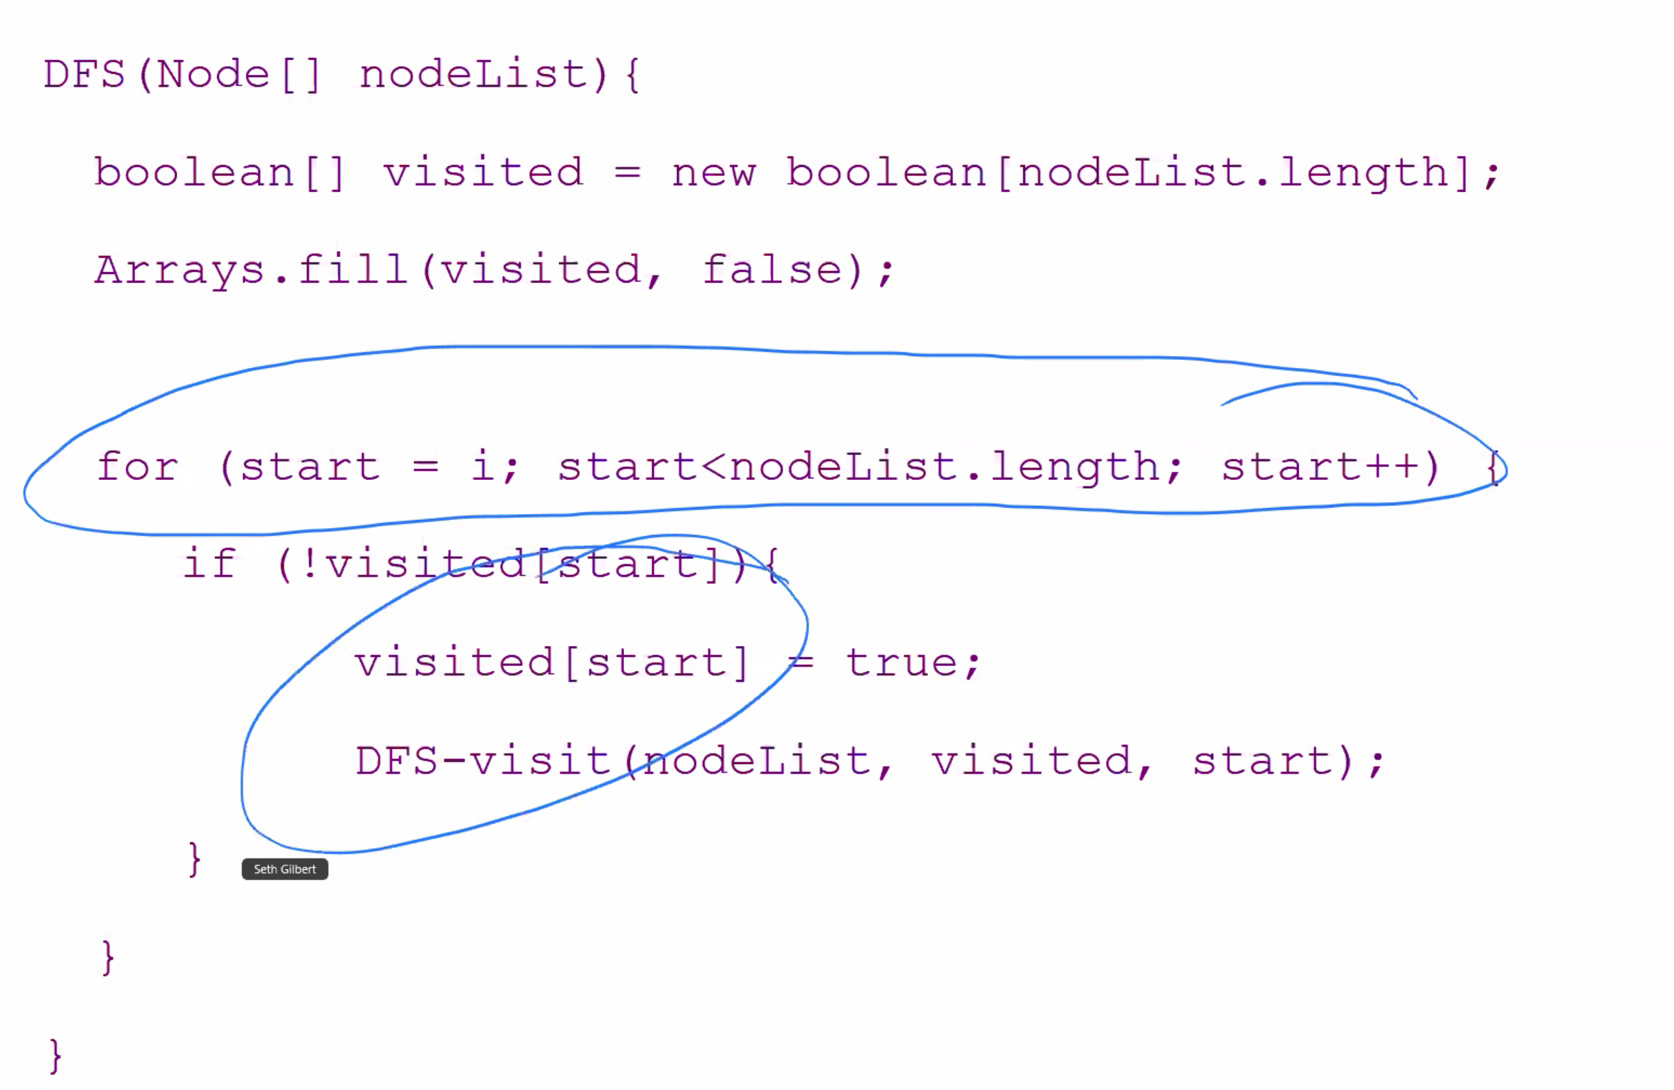
\includegraphics[scale=.11]{DFS}\\
		Implemented implicitly by call stack, doesn't return shortest path graph\\
		\textbf{Shortest Path in Weighted Graphs}\\
		Bellman-Ford - $O(VE)$, doesn't work on graphs w -ve weight cycles (NWC), can terminate early if sequence of $|E|$ relax have no effect.\\
		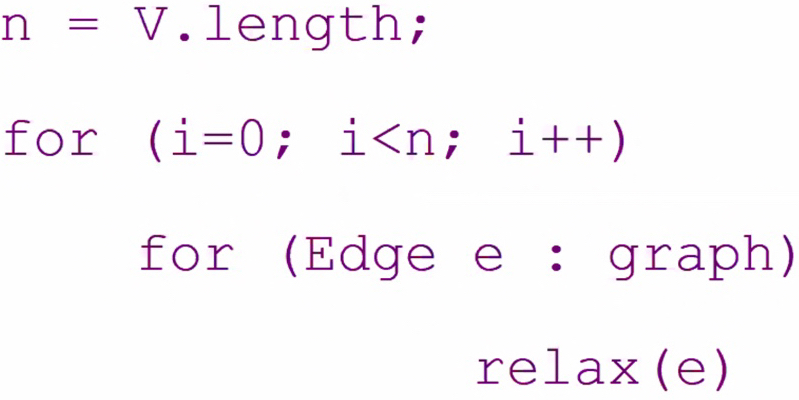
\includegraphics[scale=.12]{./assets/BF}
		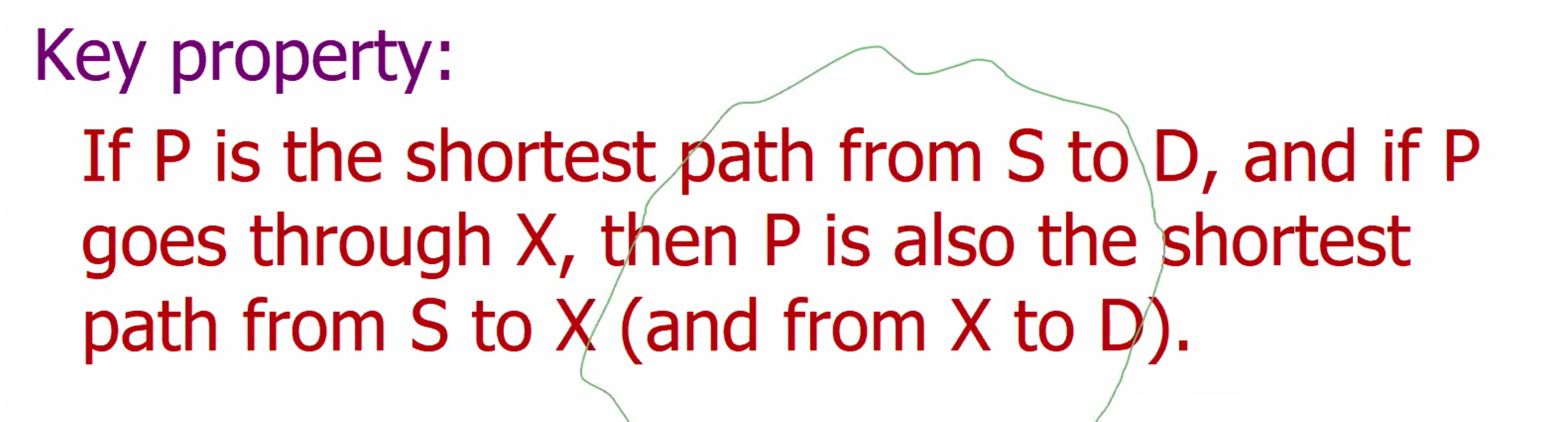
\includegraphics[scale=.1]{./assets/BF2}
		After k times, k hop estimate for nodes on shortest path is correct.\\
		Run n times to detect NWC (change on nth time)\\ 
		Dijkstra's - Relax in the right order (each edge relaxed once), works on graphs without -ve weight edges, $O(ElogV)$\\
		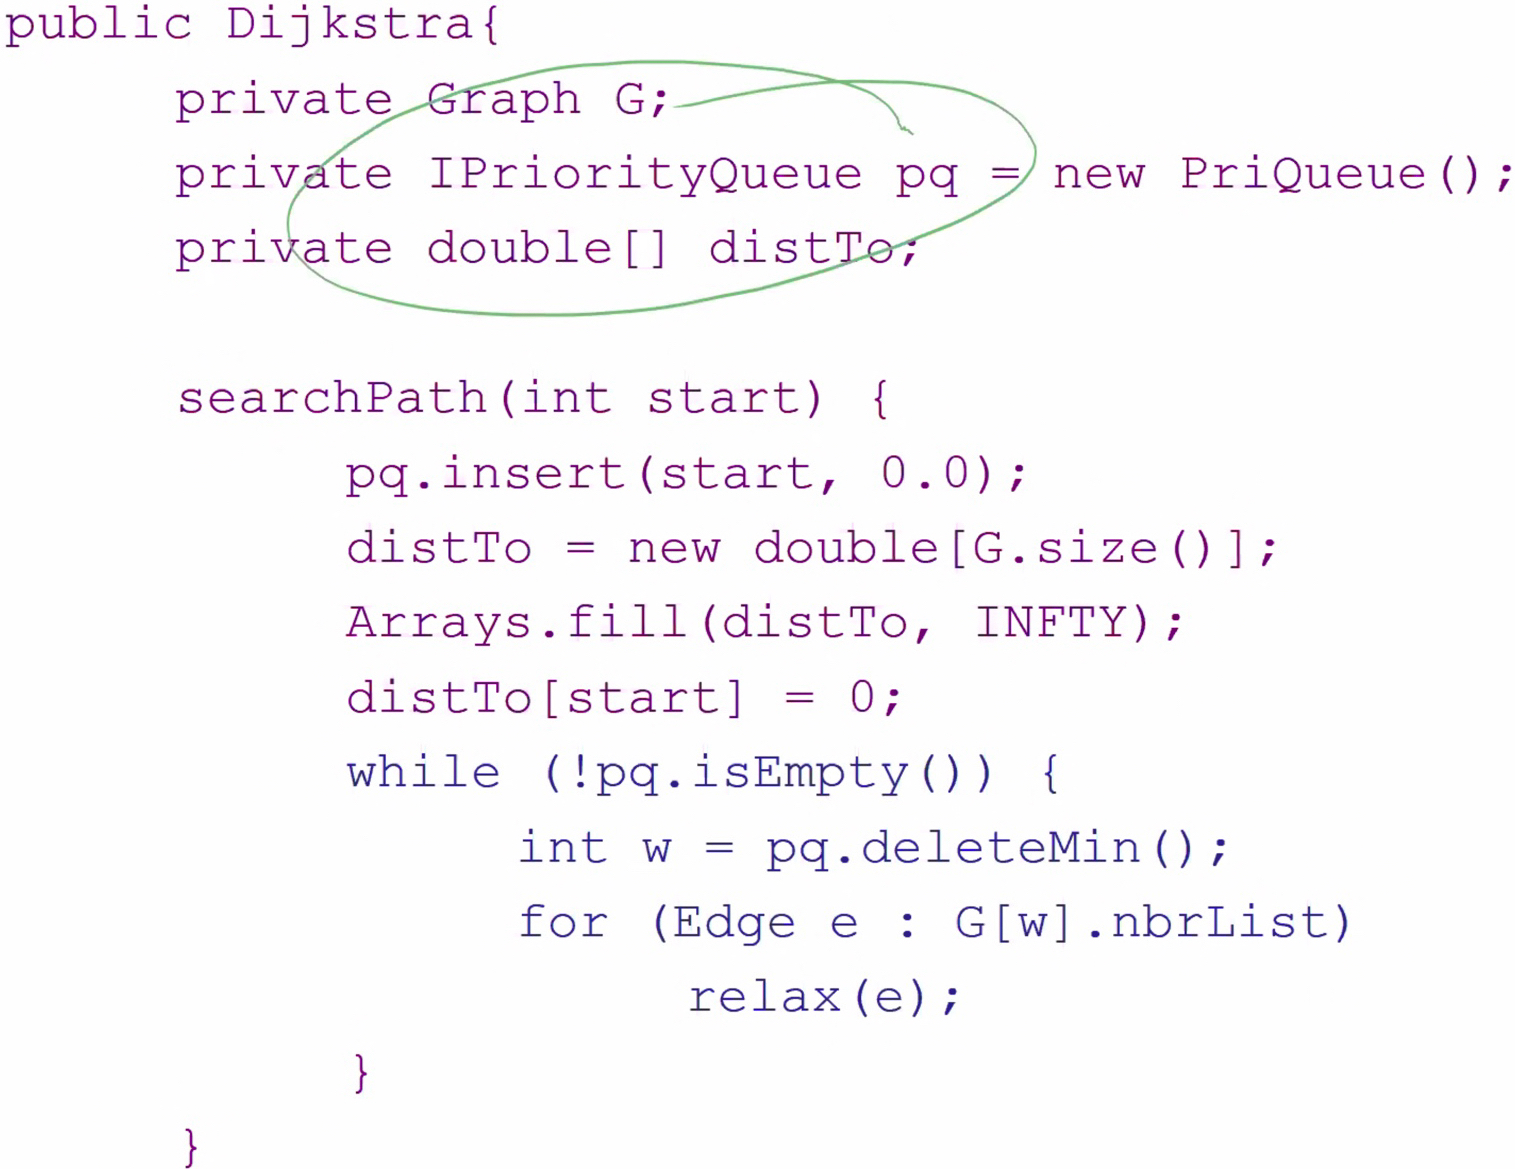
\includegraphics[scale=.09]{./assets/Dijkstra}
		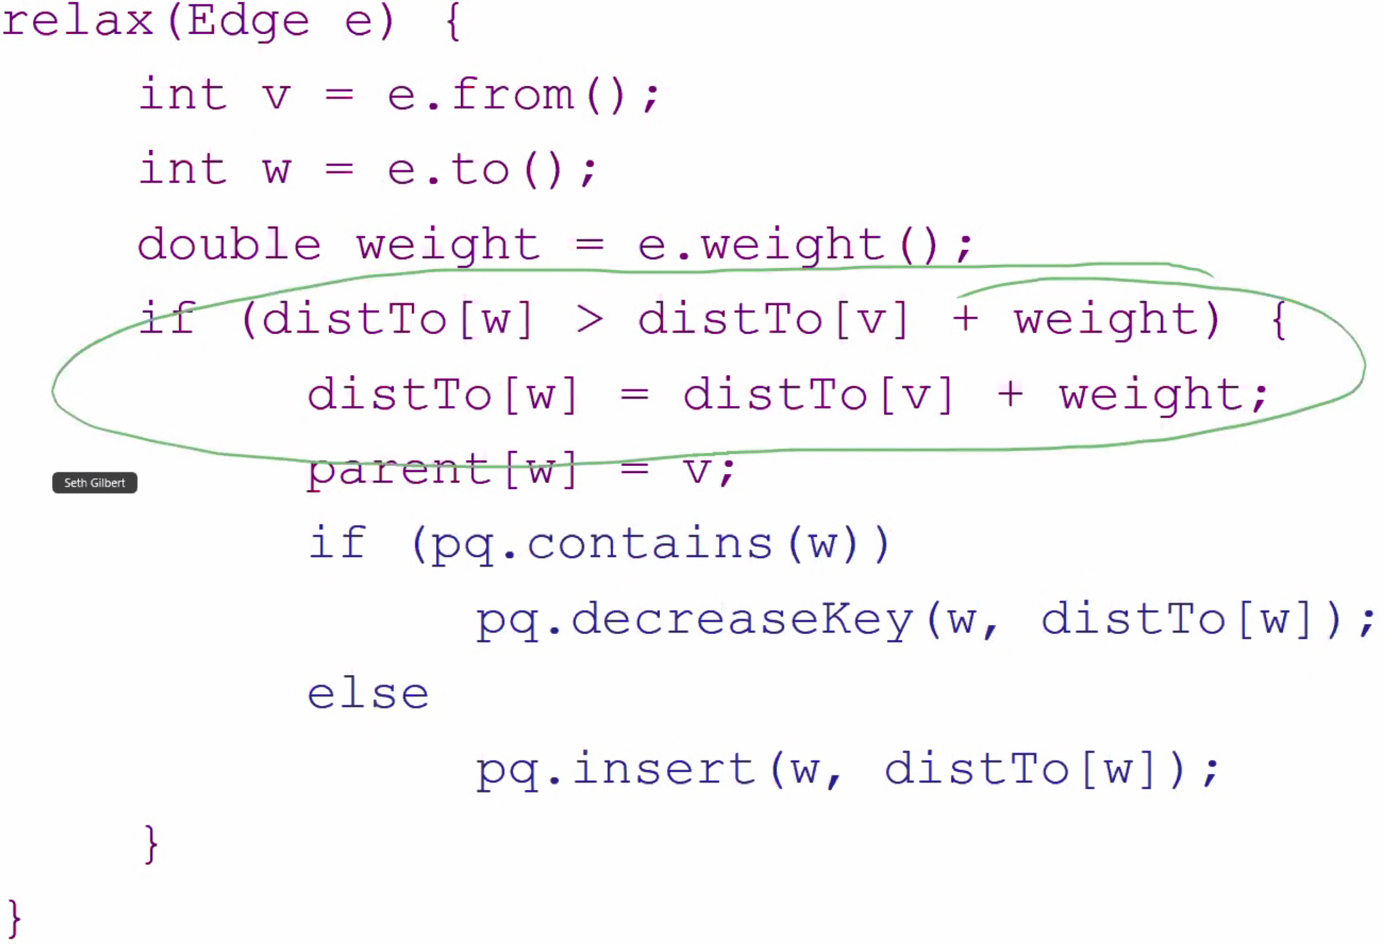
\includegraphics[scale=.09]{./assets/Dijkstra2}\\
		Main Requirement: Extending a path does not decrease its estimate.\\
		Cannot reweight graphs w -ve weight edges as paths with multiple edges will add more weight.\\
		\textbf{DAG, Topo Sort} - Only DAGs have topological orderings, converse is true\\
		1. Sequential total ordering of all nodes.\\
		2. edges only point forward.\\
		Constructing Topo Ordering - not unique, $O(V + E)$\\
		1. Post Order DFS - Process (prepend to list) each node when it is last visited\\
		\includegraphics[scale=.12]{./assets/DAG}\\
		2. Kahn's Algorithm, runtime here $O(ElogV)$ but can be done in $O(V + E)$\\
		Add nodes with no incoming edges to topo order, remove outgoing edges from that node, repeat. 
		Implement using a PQ, nodes keyed by incoming edges.\\
		\textbf{Shortest Path in DAG} - relax in topo sort order\\
		Works because if relax outgoing edge from node V, all incoming edges have been relaxed, so estimate is correct.\\
		Longest path - negate edges (can because no cycles) / modify relax function.\\
		
		{\normalsize\textbf{PQ, Heaps, Union Find Data Structure}}\\
		\textbf{Heap} - max height: $O(floor(logn))$, operations: $O(logn)$\\
		1. Heap Ordering: priority[parent] $\geq$ priority[child]\\
		2. Complete Binary Tree: Every level full except last, nodes far left \\
		Insert: insert at bottom left, bubble up until in position (swap w parent)\\
		IncreaseKey: bubble up, DecreaseKey: bubble down the larger child\\
		Delete: swap with last node, bubble up/ down as necessary\\
		ExtractMax: delete root\\
		Can be implemented with array: level order, left to right; left child = $2x + 1$, right child = $2x + 2$, parent = $floor((x-1)/2)$\\
		\textbf{HeapSort}: unsorted list to heap to sorted\\
		1. unsorted list to heap: $O(n)$, Leaves are proper heaps, recursively correct node's whos children are proper heaps by bubbling down. Base case: root\\
		2. Heap to sorted: $O(logn)$, ExtractMax and put at the end n times\\
		\textbf{UFDS - QuickFind}: Flat Trees; Find: $O(1)$, Union: $O(n)$\\
		All nodes that are in the same set are connected to same node.\\
		Find - compare root, Union - change all nodes in one set to new root\\
		\textbf{UFDS - QuickUnion}: not Flat Tree; Find $O(n)$, Union: $O(n)$\\
		Find - walk up tree of both nodes to compare roots, Union - walk up tree to roots, join one of the roots to the other\\
		\textbf{Weighted Union} - Join the smaller tree's root to the larger tree's root\\
		Max Height = $O(logn)$, tree's height only increases if joining to another tree $\geq$ itself, can happen $O(logn)$ times.\\
		\textbf{Path Compression} - When walking up a tree, set parent of each node to the root, make it flatter. Find, Union- $O(logn)$\\
		\textbf{Weighted Union w Path Compression} - Find, Union - $O(\alpha(m, n))$, m operations n objects\\
		{\normalsize\textbf{Minimum Spanning Trees}} - Prim's. Kruskals, Boruvka's\\
		Properties:\\
		1. Cannot be used to find Shortest Path\\
		2. If cut an edge of MST, get 2 MSTs (converse is not true)\\
		3. Cycle property: for every cycle, max weight edge of cycle not in MST\\
		4. False edge property: min weight edge of cycle may or may not be in MST\\
		5. Cut property: min weight edge across a cut is in MST\\
		6. Min weight adj edge of every node is in MST (6), converse not true\\
		Can reweight edges, so can MST on graph w -ve weights, MaxST: run Kruskal's in reverse.\\
		\textbf{Prim's} - $O(ElogV)$\\ 
		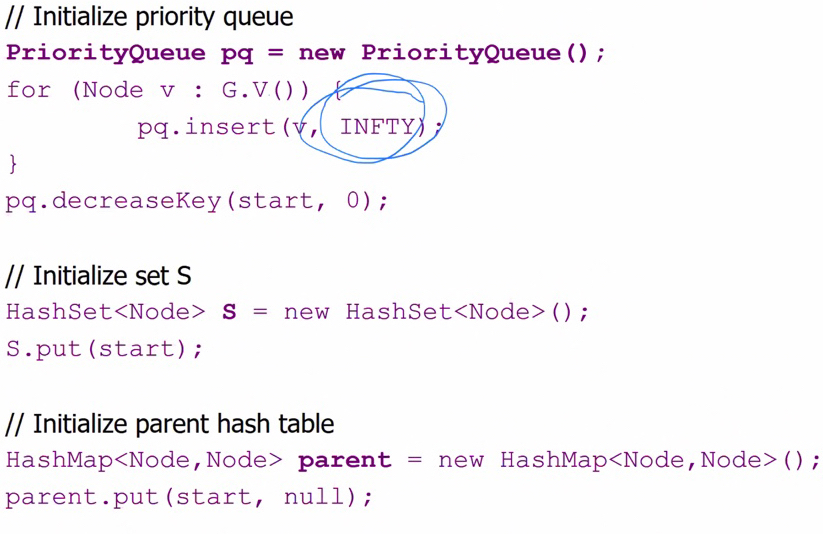
\includegraphics[scale=.2]{./assets/Prim}\\
		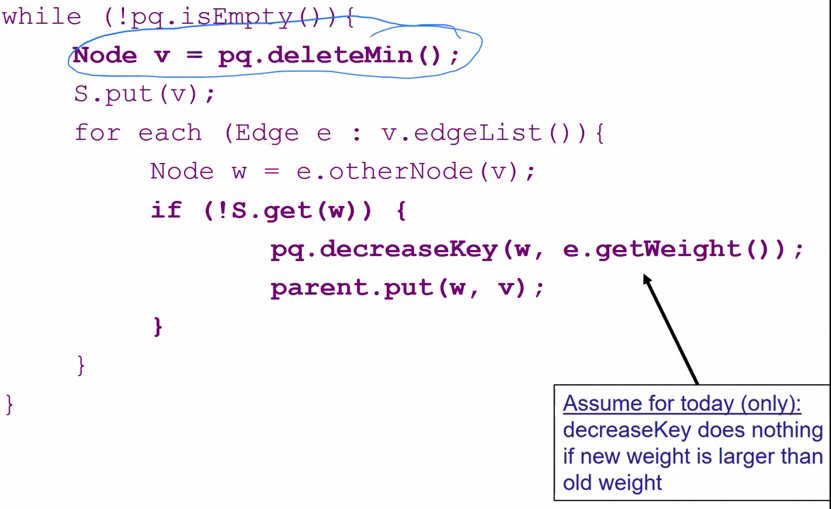
\includegraphics[scale=.18]{./assets/Prim2} Have a set $S$ of nodes, initially start node, add min weight edge across cut \{$S, V - S$\}, MST, node to $S$.\\
		\textbf{Kruskal's}: $O(ElogV)$\\
		Sort weights in ascending order.  For each edge, if both endpoints in same tree (using UFDS), then discard, if not add to MST\\ 
		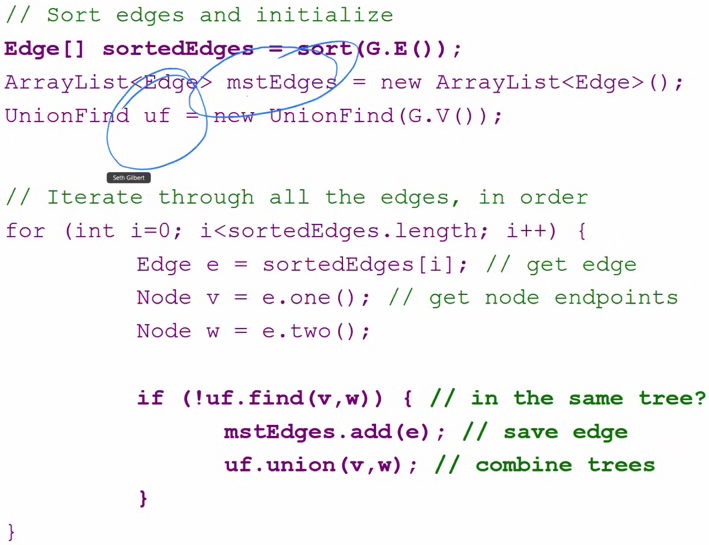
\includegraphics[scale=.22]{./assets/Kruskal}\\
		Sorting: $O(ElogE) = O(ElogV)$; Find and Union: $O(logV)$ $E$ times\\
		\textbf{Boruvka's}: $O(ElogV)$\\
		For all nodes, add min adj weight edge, adds $\geq$ $n/2$ edges each step, n is the number of connected components\\
		For each node store a component identifier: $O(V)$\\
		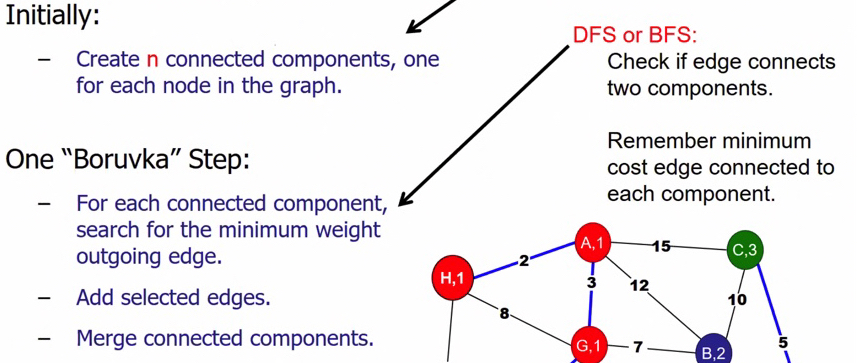
\includegraphics[scale=.21]{./assets/Boruvka}\\ 
		DFS/ BFS: $O(V + E)$, Merge CC: $O(V)$, update component IDs\\
		Each Boruvka Step: $O(V + E)$ , $O(logV)$ steps.\\
		\textbf{Steiner Tree 2 approximation}\\
		For every pair of required nodes, calculate shortest path $O(ElogV)$, Form new graph with just required nodes, run MST on new graph, Map edges back to original graph.\\
		
		{\normalsize\textbf{Dynamic Programming}}\\
		Used on problems with Optimal Substructure and Overlapping Subproblems.
		Solve problems with no dependencies first, memoize, use to solve bigger problems\\
		
		{\normalsize\textbf{Useful Stuff}}\\
		Sum of AP formula: $\frac{n}{2}(2a + (n - 1)d)$\\
		Sum of GP formula: $S_n = \frac{a(1 - r^n)}{1 - r}$\\
		$n^{log_{n}k} = k$\\
		
		Common Reccurences:\\
		$T(n) = kT(n/k) + O(n) \rightarrow O(nlogn)$\\
		$T(n) = T(n/k) + O(n) \rightarrow O(n)$\\
		
	\end{multicols*}
\end{document}